\chapter{Evaluation}
\label{chap:evaluation}

\begin{enumerate}
\item Research state-of-the-art text recognition and detection methods.

\item Generate a labeled dataset to evaluate the efficiency of the researched algorithms
   on screen content data.

\item Available datasets with subjective quality scores will be utilized to investigate
   the correlation between text recognition rates and human judgement.

\item Since most datasets do not contain textual ground truth information,
   investigate the feasibility of using recognized text from pristine images as ground truth instead.

\end{enumerate}

\section{Performance of ocr algorithms}
\label{sec:ocr_performance}

Generate a labeled dataset to evaluate the performance of the researched algorithms
on screen content data.

\begin{itemize}
\item Easy ocr generally performs well even on distorted images
\item for motion blur the performance is worse for the 2 worst quality levels for most images
\item image 4 performs better for worse quality, because gt doesn't contain text on coin
\end{itemize}

% \begin{figure}[h]
% \centering
% \includegraphics[width=0.9\textwidth]{../../data/raw/scid/DistortedSCIs/SCI04_8_1.bmp}
% \includegraphics[width=0.9\textwidth]{../../data/raw/scid/DistortedSCIs/SCI04_8_5.bmp}
% \caption{Image 4 with quality 1 and 5.}
% \label{fig:img4}
% \end{figure}

\section{Comparison against human judgement}
\label{sec:comparison_against_human_judgement}

Available datasets with subjective quality scores will be utilized to investigate
the correlation between text recognition rates and human judgement.

\subsection{Easy Ocr}
\label{subsec:easy_ocr}

\begin{itemize}
\item no clear correlation, ocr not getting substantially worse with worse quality \autoref{fig:sub29} and \autoref{fig:sub3}
\item transformation via fitted model might help
\end{itemize}

\begin{figure}[h]
\centering
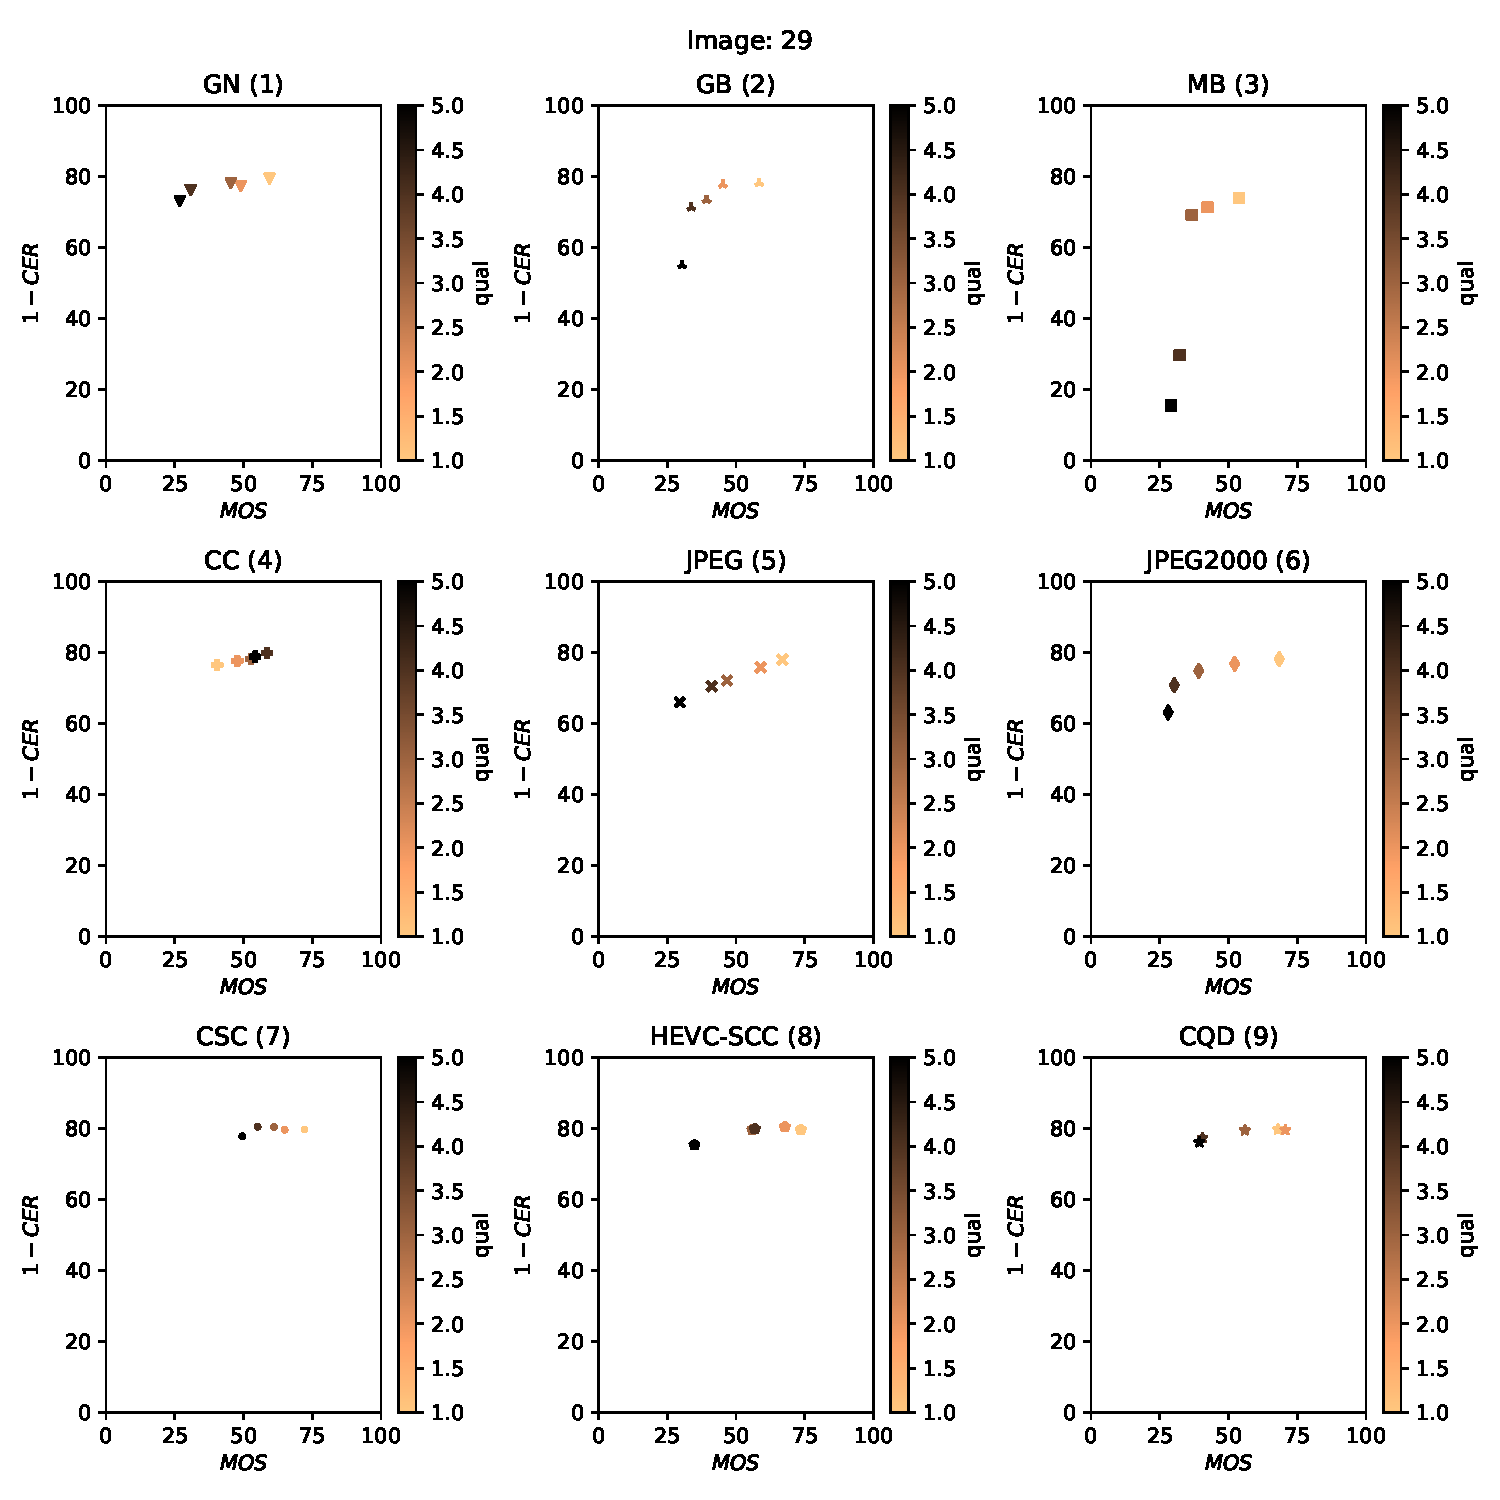
\includegraphics[width=0.9\textwidth]{../../images/analyze/mos_ter_ezocr_sub_img29.pdf}
\caption{Performance of easyocr on image 29.}
\label{fig:sub29}
\end{figure}

\begin{figure}[h]
\centering
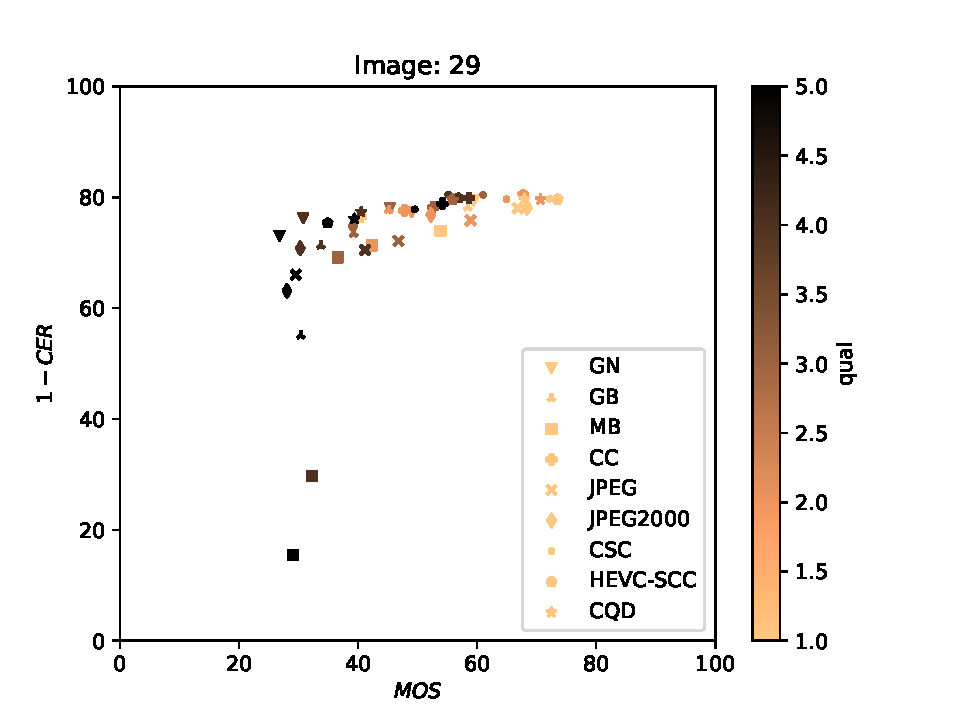
\includegraphics[width=0.9\textwidth]{../../images/analyze/mos_ter_ezocr_img29.pdf}
\caption{Performance of easyocr on image 29.}
\label{fig:img29}
\end{figure}

\begin{figure}[h]
\centering
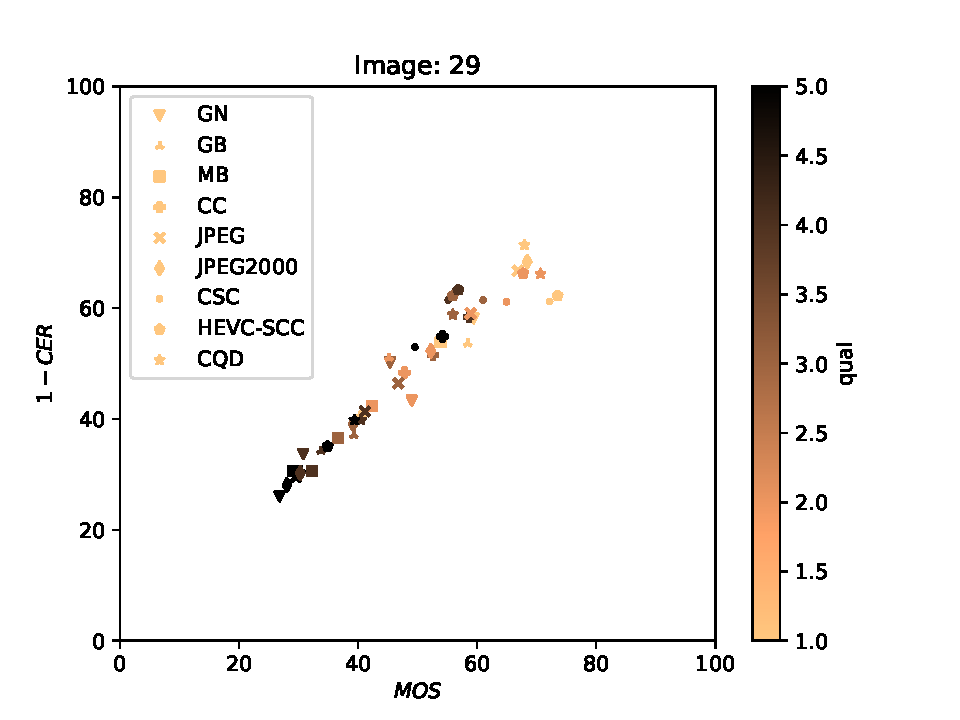
\includegraphics[width=0.9\textwidth]{../../images/analyze/mos_ter_fit_ezocr_img29.pdf}
\caption{Performance of easyocr on image 29 with fitted values.}
\label{fig:img29_fit}
\end{figure}

\begin{figure}[h]
\centering
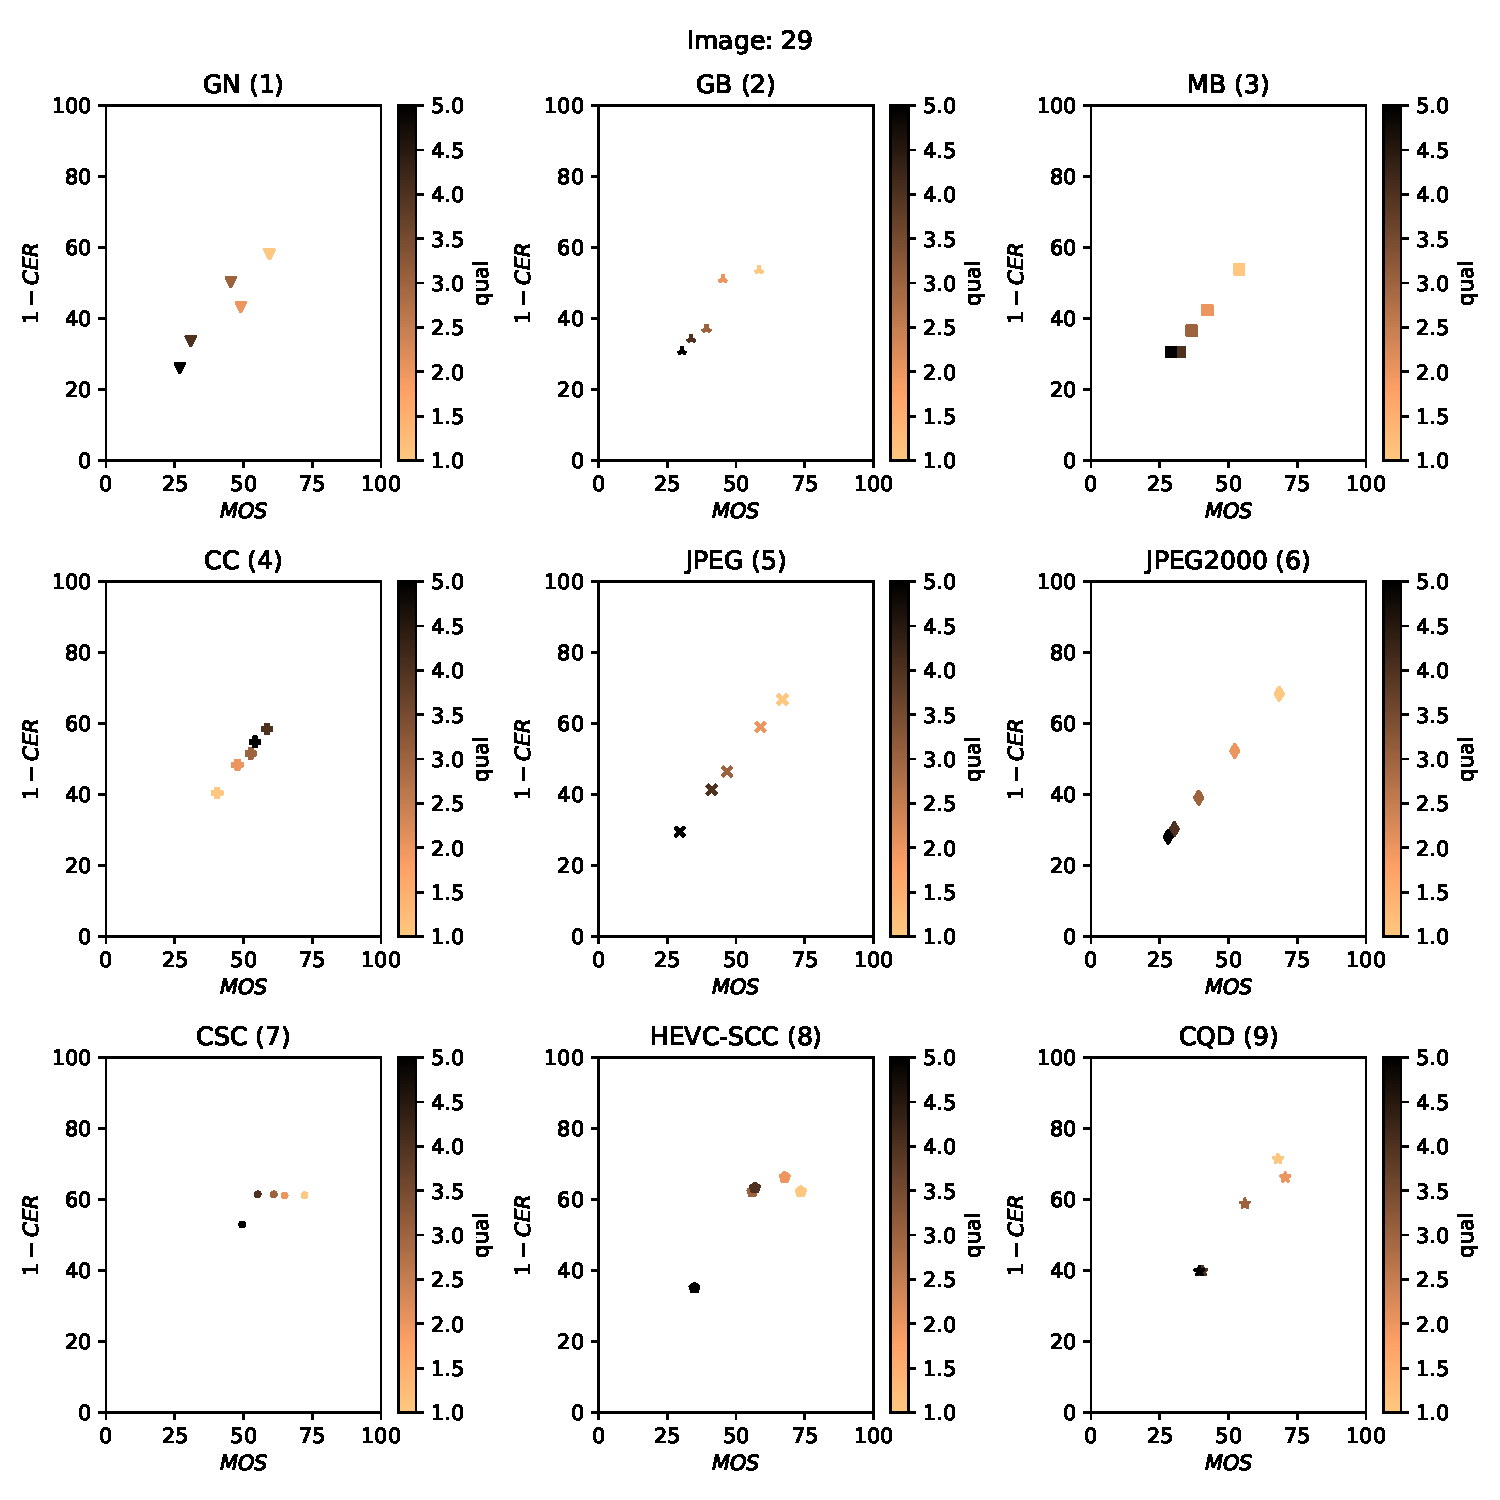
\includegraphics[width=0.9\textwidth]{../../images/analyze/mos_ter_fit_ezocr_sub_img29.pdf}
\caption{Performance of easyocr on image 29 with fitted values.}
\label{fig:sub29_fit}
\end{figure}

\begin{figure}[h]
\centering
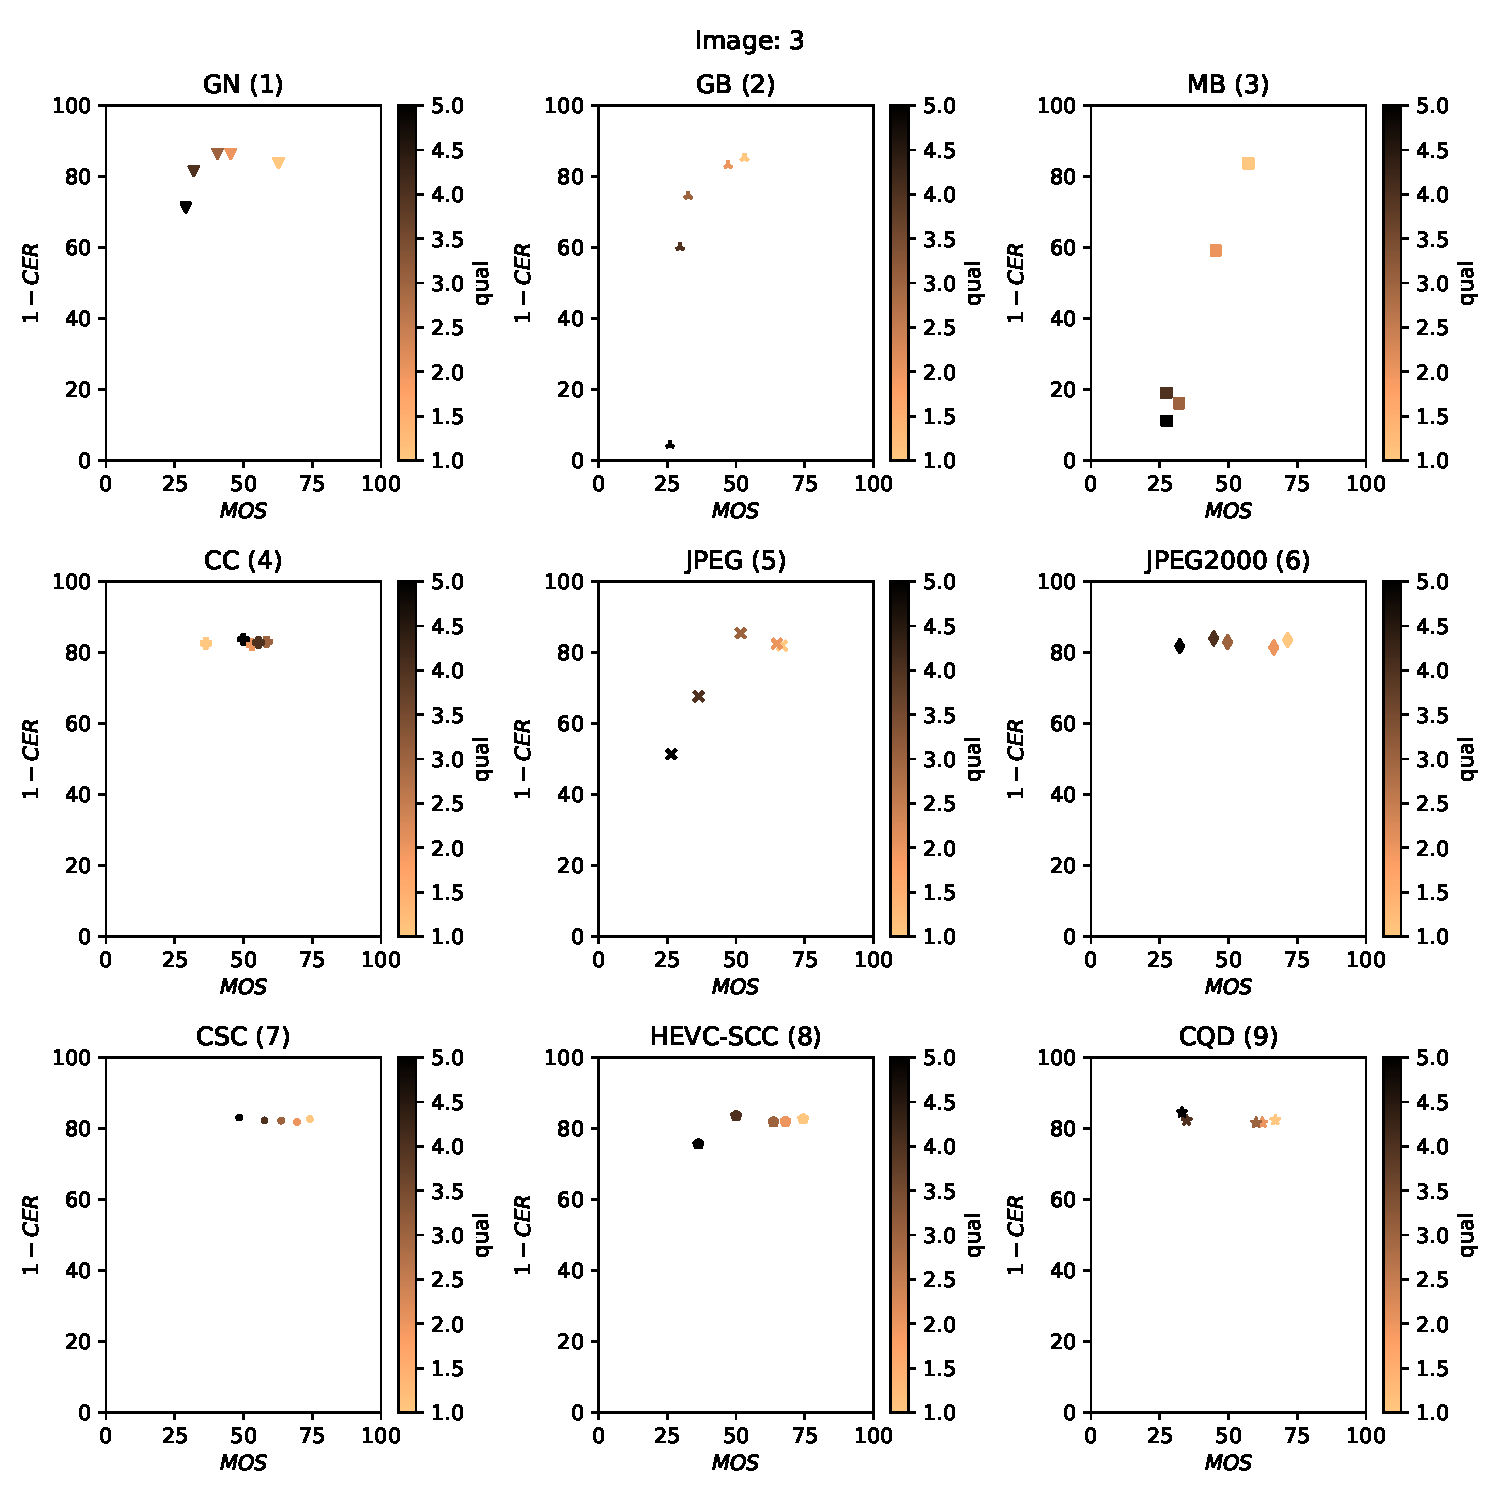
\includegraphics[width=0.9\textwidth]{../../images/analyze/mos_ter_ezocr_sub_img3.pdf}
\caption{Performance of easyocr on image 3.}
\label{fig:sub3}
\end{figure}

\subsection{Tesseract}
\label{subsec:tesseract}

\section{Usage of recognized text as ground truth}
\label{sec:usage_of_recognized_text_as_ground_truth}

Since most datasets do not contain textual ground truth information,
in a further step, Mr Hirt will investigate the feasibility of
using recognized text from pristine images as ground truth instead.

\section{Codec comparison}
\label{sec:codec_comparison}
